%!TEX root = ../template.tex
%%%%%%%%%%%%%%%%%%%%%%%%%%%%%%%%%%%%%%%%%%%%%%%%%%%%%%%%%%%%%%%%%%%%
%% chapter4.tex
%% NOVA thesis document file
%%
%% Chapter with lots of dummy text
%%%%%%%%%%%%%%%%%%%%%%%%%%%%%%%%%%%%%%%%%%%%%%%%%%%%%%%%%%%%%%%%%%%%

\typeout{NT FILE chapter4.tex}%

\chapter{Design and Application of Tooling for CMM: Fixation System Modeling}
\label{cha:dig}

In this chapter, the work previously developed by Farinha \cite{Farinha2021} will be reviewed, as it provided the foundation for the fixation system design. 
The fixture development presented here focuses exclusively on the blades of stages 6 and 7, with the understanding that the same design logic can be extended to stages 8, 9, and 10, requiring only geometric adaptations to accommodate the different dovetail profiles.
The analyses and calculations carried out throughout the development of the prototype will also be discussed, offering insight into the technical decisions, constraints, and challenges encountered during the design process.

\section{Past Work}
\label{sec:pastfix}

The design of the fixture developed in this project was guided by principles outlined by Farinha (2021), particularly those related to the functional and geometric requirements of mechanical assemblies. A fixture must ensure the complete restriction of the six degrees of freedom of the workpiece, provide stable and repeatable positioning, and allow for efficient loading and clamping without compromising accuracy. Although the author does not explicitly refer to the 3-2-1 principle, the approach described is clearly aligned with it, aiming for robust constraint through strategically positioned contact points.

Another key consideration drawn from Farinha’s work is the distinction between the locating elements, which ensure the correct positioning of the part, and the clamping elements, which apply the necessary forces to hold it during machining. The fixture must also be compatible with the specific operations required—namely milling—and with the expected geometric tolerances, avoiding distortions or positioning errors that could affect the final part.

These concepts formed the basis for the fixture proposed in this work, which was tailored to the particular geometry of the component, the machining constraints, and the overall manufacturing objectives.


\section{Fixture Design}
\label{sec:proto}

\subsection{6th and 7th Stage Blade Geometry Assessment}

Instead of designing a dedicated fixture for each stage, it was verified that the dovetail geometries of the blades from the 6th and 7th stages are sufficiently similar to allow the use of a single fixture for both.
Figure~\ref{fig:bladecompare} shows the overlap between the dovetails of a 6th stage blade (dark brown) and a 7th stage blade (beige), confirming the geometric compatibility.
As a result, a single fixture will be designed to accommodate both stages.

\begin{figure}[H]
    \centering
    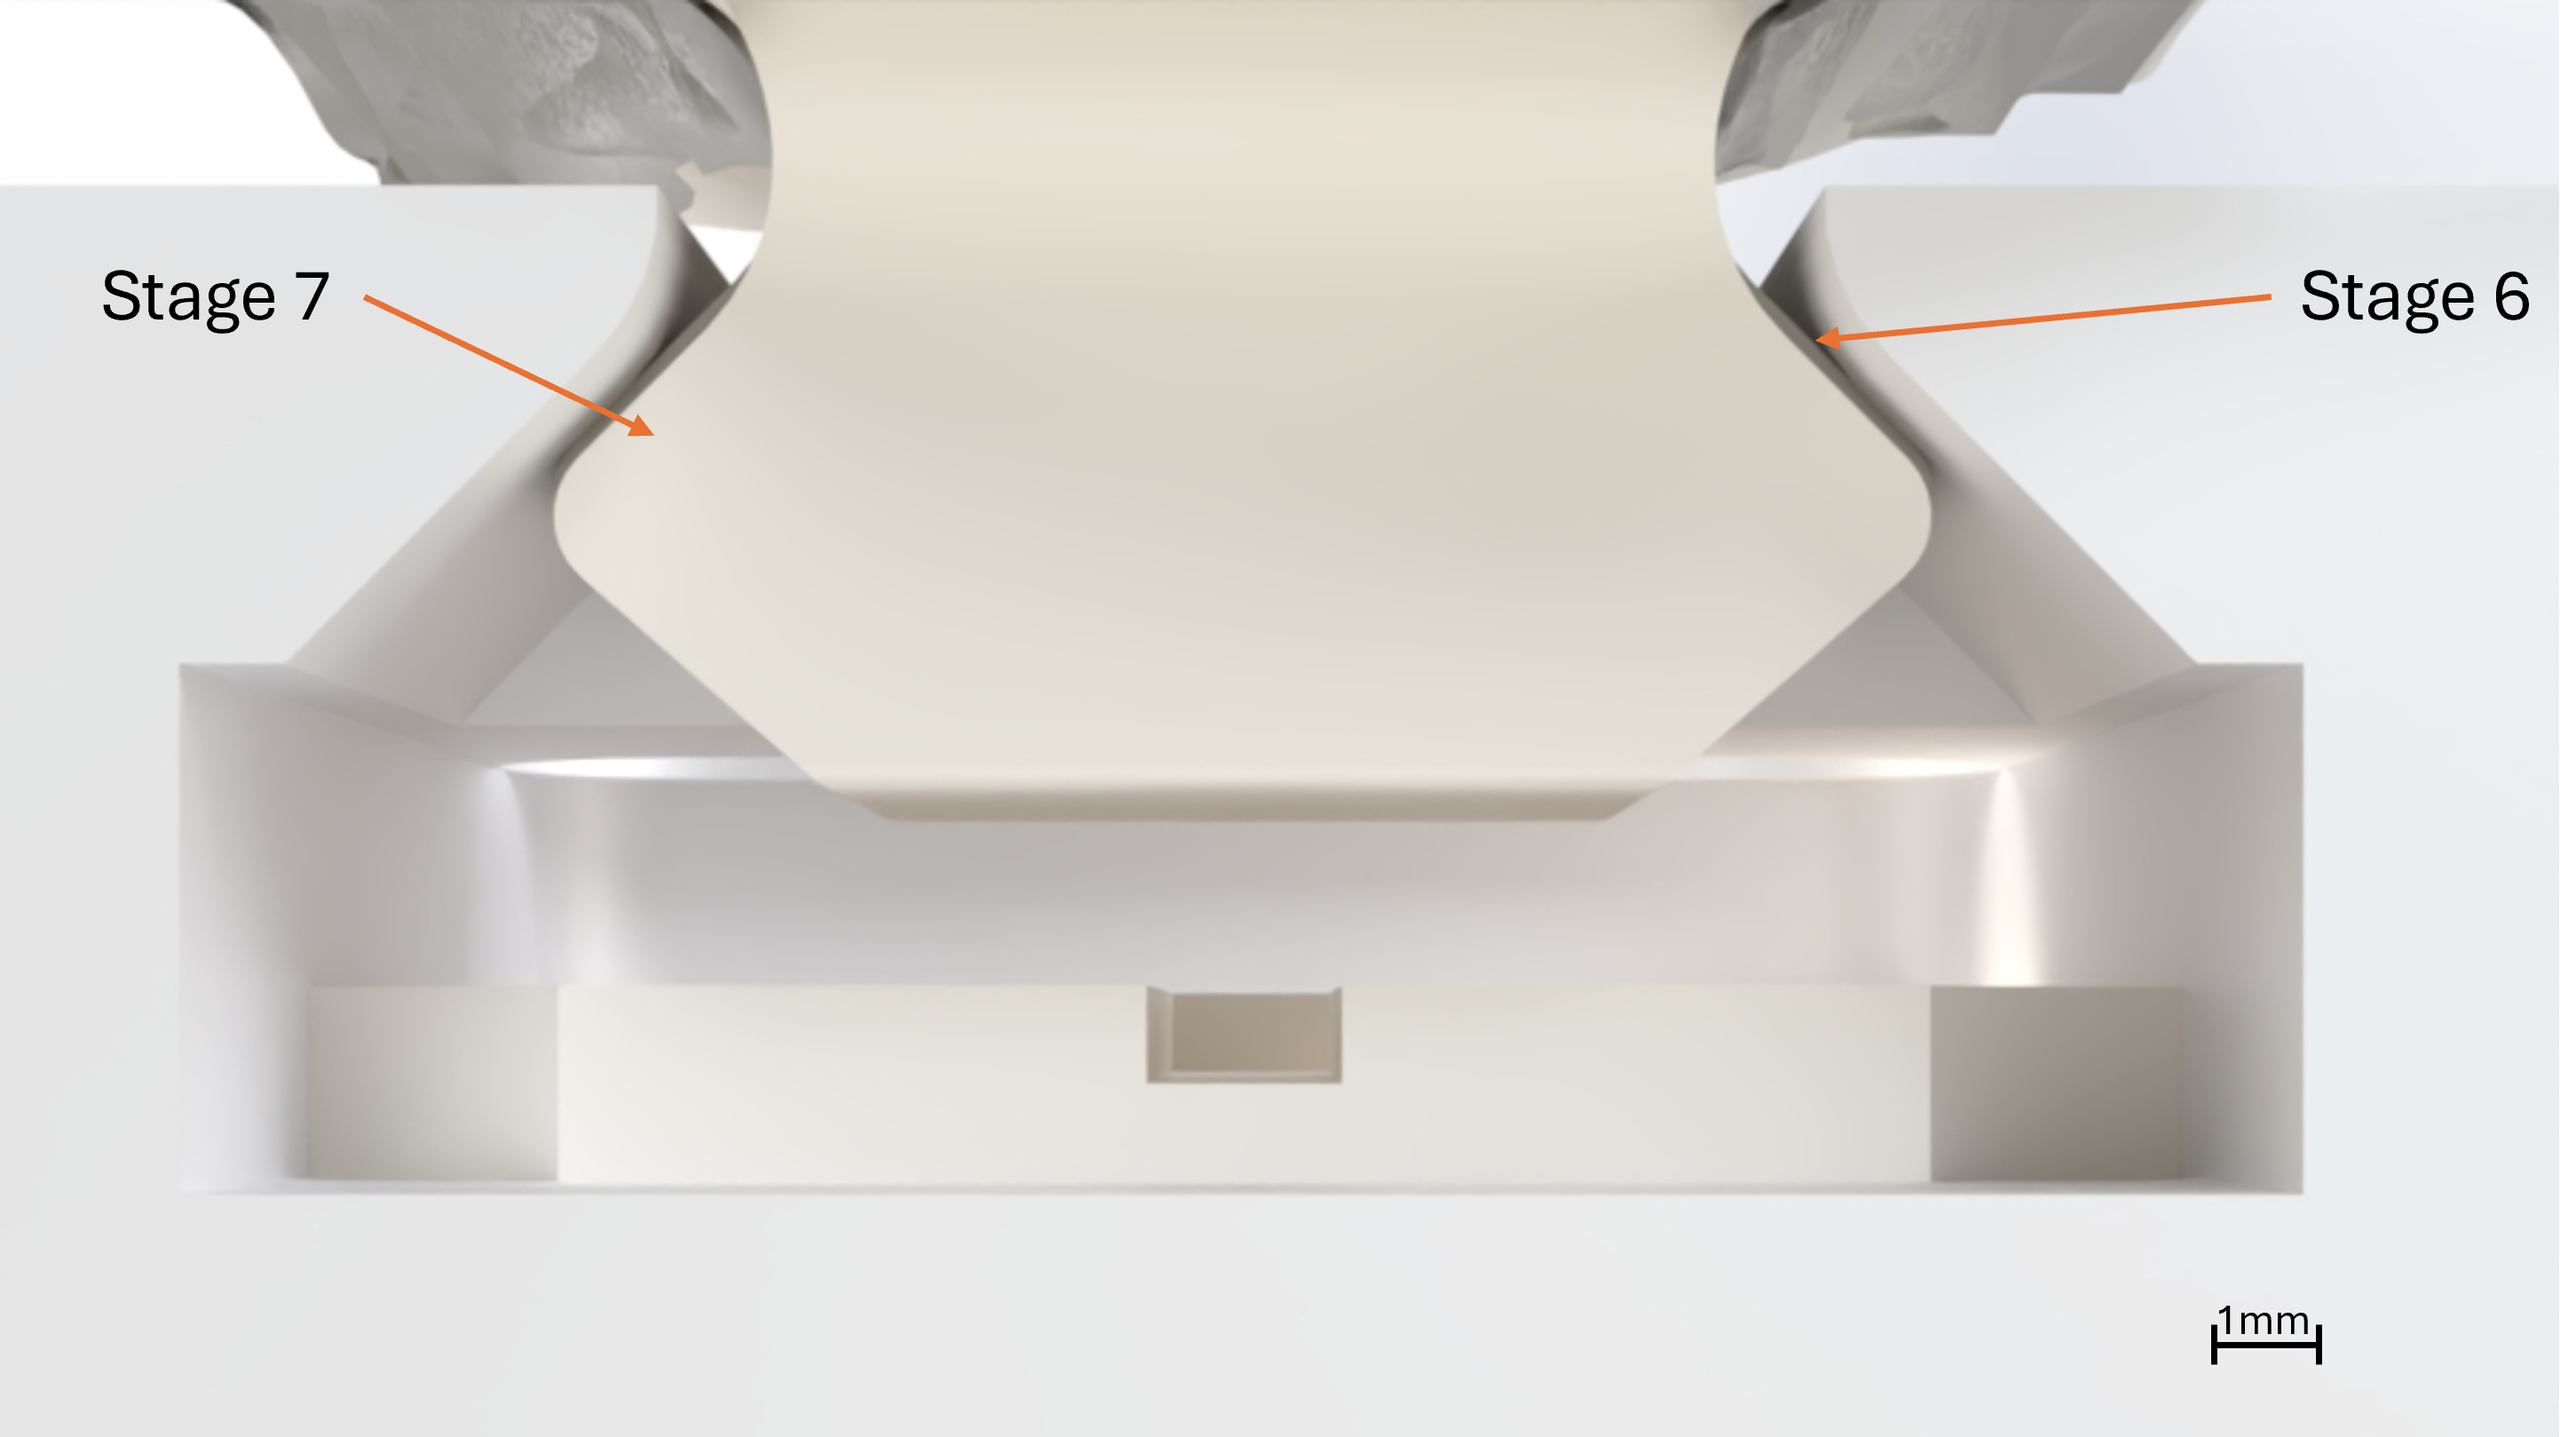
\includegraphics[width=0.65\textwidth]{bladecompare}
    \caption{Overlay of dovetail profiles from the 6th stage and 7th stage blades.}
    \label{fig:bladecompare}
\end{figure}

\subsection{Blade Fastening System}

The fixture was developed to constrain the HPC blade in the Y and Z directions through contact with two precisely machined blocks, both shaped to match the geometry of the blade’s dovetail. 
This configuration ensures consistent vertical and lateral positioning, as illustrated in Figure~\ref{fig:fixture_exploded}, which presents an exploded view of the main components.

The top contact block interfaces with defined regions on the blade. 
These surfaces were selected to avoid functional zones while still providing the necessary mechanical stability. 
Figure~\ref{fig:contact_surface_blade} shows the contact areas on the blade itself, and Figure~\ref{fig:contact_surface_tool} highlights the corresponding surfaces on the fixture.

\begin{figure}[H]
    \centering
    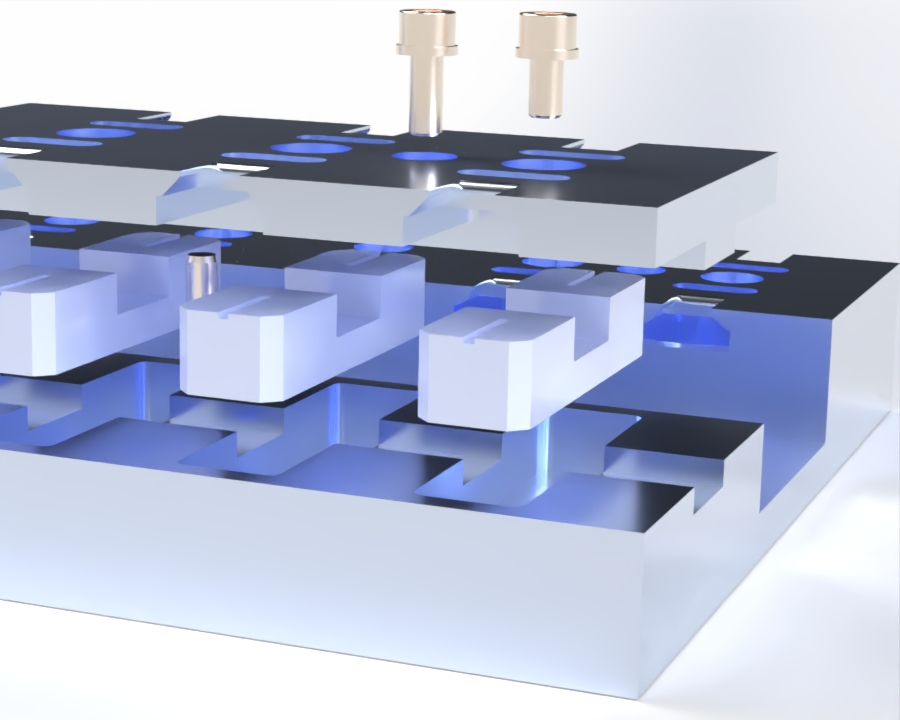
\includegraphics[width=0.75\textwidth]{fixture_exploded}
    \caption{Exploded view of the fixture showing the base plate, bottom support block, top contact block, and clamping element. The geometry of the contact surfaces is adapted to the blade’s platform and dovetail profile.}
    \label{fig:fixture_exploded}
\end{figure}

\begin{figure}[H]
    \centering
    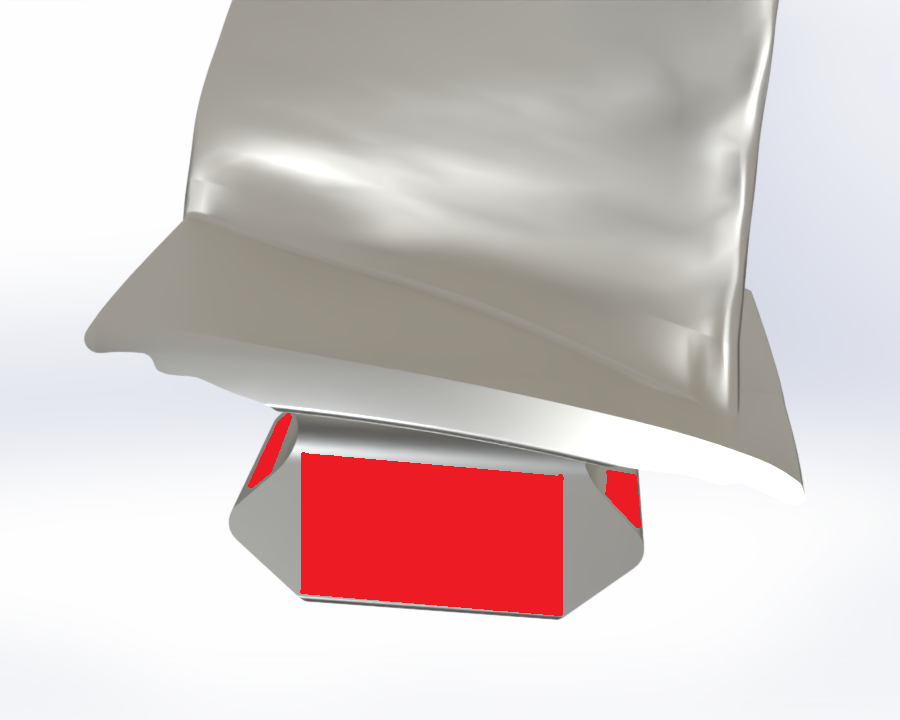
\includegraphics[width=0.5\textwidth]{contact_surface_blade}
    \caption{Contact surfaces on the blade that interface with the top contact block of the fixture.}
    \label{fig:contact_surface_blade}
\end{figure}

\begin{figure}[H]
    \centering
    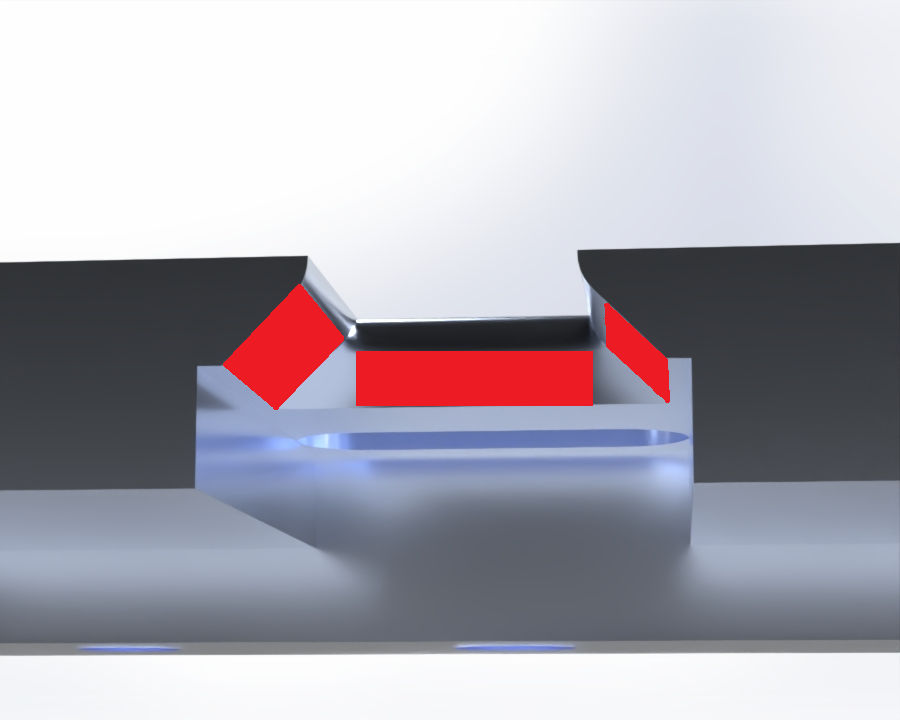
\includegraphics[width=0.5\textwidth]{contact_surface_tool}
    \caption{Contact surfaces on the top contact block of the fixture, matching the geometry of the blade.}
    \label{fig:contact_surface_tool}
\end{figure}

Although the blade is not geometrically constrained along the X axis, a clamping element actuated by a screw applies a downward force that securely locks the blade in place. 
This pressure piece ensures immobilization during the measurement process. 
Small variations in the X position between blades are absorbed during the CMM alignment stage, since the coordinate system is redefined based on the actual part position before each measurement.

To prevent potential blade slippage during probing, a solution previously proposed and validated by Farinha (2021) was directly applied. 
In his prototype, it was observed that the combination of polished aluminium and titanium resulted in low friction, allowing the blade to move under small applied forces. 
To overcome this, Farinha recommended the use of a thin rubber strip at the contact surfaces. This increases the local friction coefficient and eliminates the need for high clamping forces. 
Given its proven effectiveness and its common use in MRO procedures, this solution was incorporated into the present fixture design by applying the rubber only on the relevant angular surfaces of the top contact block that interface with the blade.

\subsection{Blade Spacing }




\subsection{Fixture Threading and Transportation Features}

\subsection{Fastening Feature of the Fixture with CMM's TAble}